\chapter{Une méthode de composition dynamique des services Web
  sémantiques utilisant Neo4j}
\label{ch:approach}

\section*{Introduction}
\addcontentsline{toc}{section}{Introduction} \markboth{INTRODUCTION}{}

\newpage
\section{Reformulation du problème}
\label{sec:reformulation}

Cette section a pur but d'introduire les notions de base ainsi que les
notations et terminologies employées dans la suite de ce
chapitre. Nous présentons une formulation mathématique de notre
problème principal, à savoir \textit{la composition des servies Web}
sous forme d'un problème de recherche du plus court chemin dans un
graphe orienté .\bigskip

Chaque service web peut contenir les définitions de différentes
opérations \acrshort{wsdl} identifiables par leurs noms et leurs
paramètres. Pour des raisons de simplicité, nous supposons que chaque
service Web représente une seule opération.\medskip

\begin{mydef}[\textbf{Service Web}]
  Un Service Web $S$ est un 2-tuple $\mathpzc{<I,O>}$, où
  $\mathpzc{I}=\{I_0, \dots, I_n\}$ désigne l'ensemble des paramètres
  d'entrée, $\mathpzc{O}=\{O_0, \dots, O_m\}$ l'ensemble des
  paramètres de sortie.
\end{mydef}

%!TEX root = ../../main.tex
\begin{figure}[h]
    \centering
    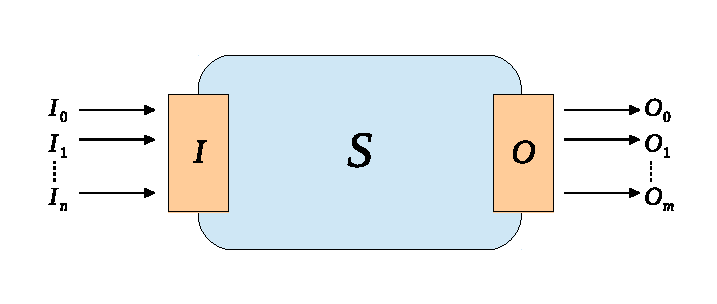
\includegraphics[width=0.65\textwidth]{figs/ch3/ws.eps}
    \caption{Un service Web atomique.}
    \label{fig:ch3/ws}
\end{figure}
%%% Local Variables:
%%% mode: latex
%%% TeX-master: "../../main"
%%% End:


Dans notre approche proposée, nous supposons que chaque service est
décrit par un document \acrshort{owls} qui possède un seule processus
atomique, et que chaque paramètre est lié à un concept dans
l'ontologie \acrshort{owl} du domaine.\medskip

\begin{mydef}[\textbf{Annuaire des services Web}]
  Un annuaire des services Web est un ensemble
  $\mathpzc{R} =\{\mathit{S_0}, \mathpzc{S_1}, \dots,\mathit{S_n}\}$
  des services Web disponibles, où chaque
  $\mathpzc{S} \in \mathpzc{R}$ est un service Web.
\end{mydef}

Afin de trouver un service composite exécutable à partir d'un annuaire
de services Web, un utilisateur doit fournir une requête de
composition.\medskip

\begin{mydef}[\textbf{Requête}]
  Une requête $\mathpzc{Q}$ est un 2-tuple $\mathpzc{<I_Q, O_Q>}$.
  $\mathpzc{I_Q}$ désigne la liste des paramètres d'entrée fournis par
  l'utilisateur (ou par un service client) et $\mathpzc{O_Q}$
  représente la listes des paramètres requis (sorties).
\end{mydef}

Afin de découvrir et sélectionner un service Web composite suite à une
requête de composition, les services référencés dans un annuaire
doivent être structurés dans un graphe orienté modélisant toutes les
relations de dépendance fonctionnelle possibles pour permettre de
réaliser un \textit{Matching} horizontal \ref{sec:matching} (la figure
\ref{fig:ch4/gd}) entre les services disponibles deux à deux.\medskip

%!TEX root = ../../main.tex
\begin{figure}[h]
    \centering
    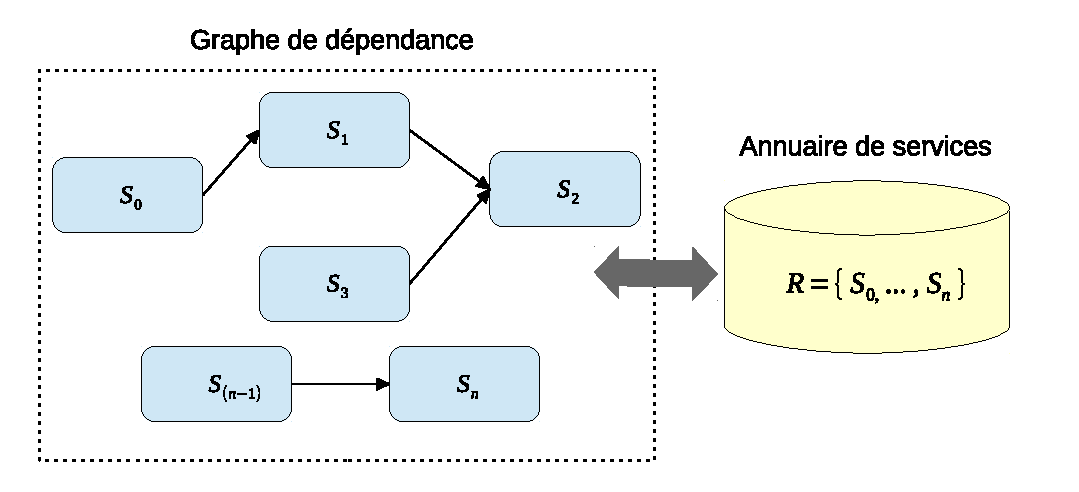
\includegraphics[width=1.1\textwidth]{figs/ch3/gd.eps}
    \caption{Graphe de dépendance $\mathpzc{GD}$ entre les services
      Web d'un annuaire $\mathpzc{R}$.}
    \label{fig:ch4/gd}
\end{figure}
%%% Local Variables:
%%% mode: latex
%%% TeX-master: "../../main"
%%% End:


\begin{mydef}[\textbf{Graphe de dépendance}]
  Un graphe de dépendance $\mathpzc{DG}$ est un ``graphe orienté et
  acyclique'' $\mathpzc{DG}=<\mathpzc{R}, \mathpzc{L}>$ qui modélise
  toutes les relations de dépendance fonctionnelle possibles entre les
  services Web disponibles dans un annuaire $\mathpzc{R}$. Il existe
  une relation
  $\mathit{L_{ij}}=(\mathit{S_i}, \mathit{S_j}) \in \mathpzc{L}$ si et
  seulement s'il existe une relation de dépendance fonctionnelle entre
  $\mathit{S_i}$ et $\mathit{S_j}$, où
  $\{\mathit{S_i, S_j}\} \subset \mathpzc{R}$.\medskip
\end{mydef}

L'approche proposée consiste à construire le graphe de dépendance à
priori (\textit{Offline}) et le sauvegarder dans une base de données
graphe (\textit{Neo4j}). Suite à une requête $\mathpzc{Q}$, un
sous-graphe $\mathpzc{G}$ est extrait, qui correspond à un plan de
composition exécutable $\mathpzc{P}$ d'un service Web composite
satisfaisant.\medskip

%!TEX root = ../../main.tex
\begin{figure}[h]
    \centering
    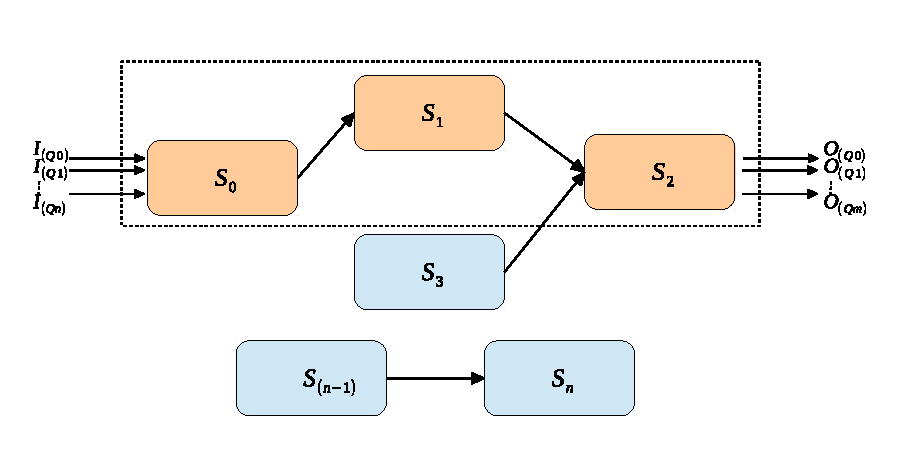
\includegraphics[width=1\textwidth]{figs/ch3/composition-plan.eps}
    \caption{Un service Web composite avec le plan de composition correspond.}
    \label{fig:ch3/composition-plan}
\end{figure}
%%% Local Variables:
%%% mode: latex
%%% TeX-master: "../../main"
%%% End:


\begin{mydef}[\textbf{Plan de composition}]
  Un plan de composition $\mathpzc{P}$ est un sous-graphe
  $\mathpzc{G \subset DG}$ \textbf{``connexe''} d'un graphe de
  dépendance $\mathpzc{DG}$, tel que $\mathpzc{G=(R_Q,L_Q)}$ décrit le
  flux de données/contrôles d'exécution d'un ensemble de services Web
  atomiques $\mathpzc{R_Q \subset R}$ engagés dans un processus de
  composition. Il existe un lien de dépendance fonctionnelle
  (\textit{Link}) $\mathit{L_{Q_{ij}}} \in \mathpzc{L_Q}$ tel que
  $\mathit{L_{Q_{ij}}} = (S_i, S_j)$ si l'exécution d'un service
  $\mathit{S_j}$ dépend d'un ou plusieurs paramètres de sortie de
  $\mathit{S_i}$.\medskip
\end{mydef}

\begin{mydef}[\textbf{Service Web composite}]
  Un service Web composite $\mathpzc{S_Q}$ est un service Web
  exécutable composé de $n \geq 1$ services atomiques
  $\mathit{S_{0 \leq i \leq n}} \in \mathpzc{R_Q}$ tel que l'exécution
  d'un tel service correspond à l'exécution d'un plan de composition
  $\mathpzc{P}$ décrit par un graphe de dépendance
  $\mathpzc{G = <R_Q,L_Q>}$ suite à une requête $\mathpzc{Q}$.\medskip
\end{mydef}

La figure \ref{fig:ch3/composition-plan} montre un service Web
composite
$\mathpzc{S_Q} = <\mathit{\{I_0, \dots, I_n\}}, \mathit{\{O_0, \dots,
  O_m\}}>$
correspondant à un plan de composition $\mathpzc{P}$ représenté par un
graphe de dépendances connexe $\mathpzc{G =<R_Q,L_Q>}$, tel que
$\mathpzc{R_Q = \{S_0, S_1, S_2\}}$ et
$\mathpzc{L_Q = \{(S_0, S_1), (S_1, S_2)\}}$.\medskip

Une service Web composite $\mathpzc{S_Q = <I_S, O_S>}$ est créer et
exécuter suite à une requête de composition $\mathpzc{Q=<I_Q, O_Q>}$.
Deux conditions nécessaires et suffisantes pour que $\mathpzc{S_Q}$
satisfasse $\mathpzc{Q}$:\medskip

\begin{enumerateRoman}
\item L'interface d'entrée $\mathpzc{I_S}$ est subsumé par
  $\mathpzc{I_Q}$ ($\mathpzc{I_S \subseteq I_Q}$).

\item L'interface de sortie $\mathpzc{I_Q}$ est subsumé par
  $\mathpzc{I_S}$ ($\mathpzc{O_Q \subseteq O_S}$).\medskip
\end{enumerateRoman}
\enddescription

La relation ``$\subseteq$'' de \emph{``subsomption`''} entre les
interfaces d'\emph{entrée/sortie} sera abordée dans la
section~\ref{sec:matching}.

\begin{mydef}[\textbf{Problème de composition}]
  Étant donné $\mathpzc{R}$ un annuaire des services Web et
  $\mathpzc{Q}$ une requête, Le problème de composition
  $\mathpzc{WCP=<R,Q>}$ consiste à trouver un plan de composition
  exécutable et optimal $\mathpzc{P}$ associé au service Web composite
  $\mathpzc{S_Q}$ satisfaisant la requête $\mathpzc{Q}$.
\end{mydef}

%!TEX root = ../../main.tex
\begin{figure}[h]
    \centering
    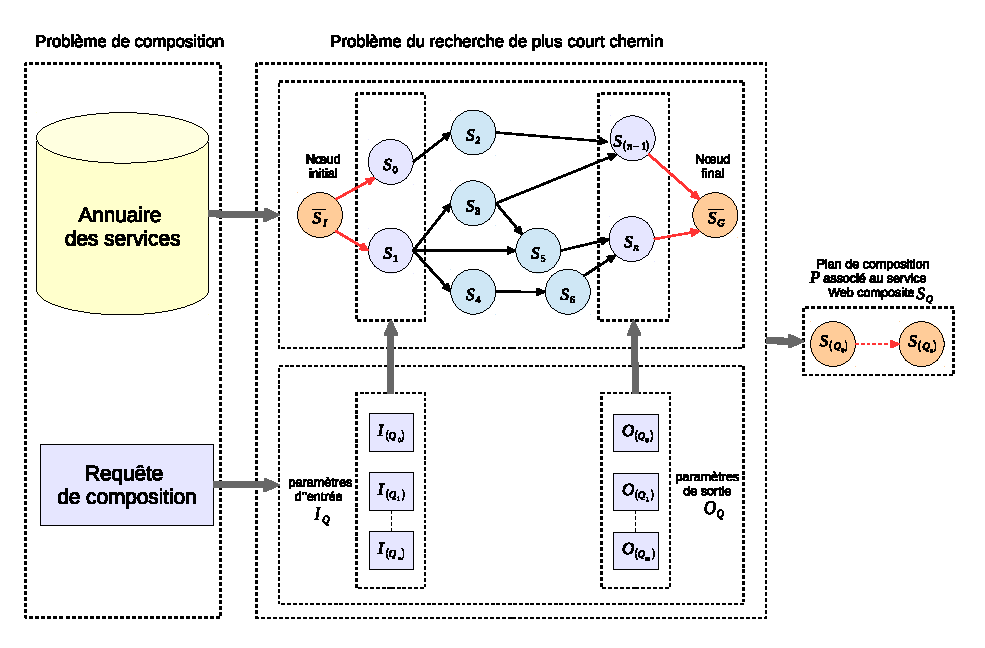
\includegraphics[width=1.15\textwidth]{figs/ch3/reformulation.eps}
    \caption{Reformulation du problème.}
    \label{fig:ch3/reformulation}
\end{figure}
%%% Local Variables:
%%% mode: latex
%%% TeX-master: "../../main"
%%% End:


\newpage
\section{Architecture générale}
\label{sec:proposition}

\section{Matching de services Web atomiques}
\label{sec:matching}

\section{Construction du graphe de dépendance}
\label{sec:dg}

\section{Découverte de services Web composites}
\label{sec:composite-discovery}
\section*{Conclusion}
\label{sec:conclusion}
\addcontentsline{toc}{section}{Conclusion} \markboth{CONCLUSION}{}


%%% Local Variables:
%%% mode: latex
%%% TeX-master: "../main"
%%% End:
